\section{Feature Learning}
	
	\label{sec:allFeat}
  Features used in our system are categorized to three types: activity features, user-related features, and course-related features, which are defined as $\mathbf{Feat}_a$, $\mathbf{Feat}_u$ and $\mathbf{Feat}_c$, respectively. Activity features mainly include users' learning behaviors, which are extracted from user historical activity sequence. User- and course-related features are mainly from user-course enrollment graph.
  %and these two sets of features are mainly used to capture user and course information from the perspective of user and course respectively.
  
	%And, in order to capture the context information for MOOC users, a series of user-related features and course-related features are  also used in our framework. 
	\subsection{Activity Features}
	
	\label{sec:activityFeat}
This set of features are from user historical activity logs. We employ both statistical methods and a Long Short-Term Memory (LSTM) framework to learn user behavior patterns. This part of features are represented by $\mathbf{Feat}_{a}$. \\\\
\noindent \textbf{Statistics Features}
\begin{enumerate}
	\item{Activity Count/Ratio:} For each enrollment $(u,c)$, we calculate the number and ratio for each type of activities in table \ref{ResourceAction}. 
	\item{Activity Temporal Statistics:} The whole duration time of a course is divided by weeks, and the activity counts and statistics(including \emph{max, min, stdev, median}) in different weeks are used as features.
	\item{Activity Count in Hours Per Day:} We calculate user activity count for each hour in a day (24 hours).
	\item{Activity Count in Day Per Week:} We compute user activity count for each day in a week (5 weekdays + 2 weekends).
	\item{Activity N-gram Count/Ratio:} The N-grams of activity sequence is used to capture the correlations between neighbor activities. We employ N-gram activity count and ratio as the N-gram features.
	\item{Engagement Style:} Following the taxonomy of engagement introduced by Anderson et al. \cite{Anderson:2014:EMO:2566486.2568042ß}, we use the $\emph{assignment fraction} = \frac{ \emph{watching video \#}}{ \emph{complete assignment \#}}$ to represent user's engagement pattern.
	\item{Learning Time Span:} A user's learning time span is the duration between a user's first visit time and her last visit time on a course.  
	
	\item{Effective Learning Time:} The \emph{effective learning time} introduced by Qiu et al. \cite{Qiu:2016:MPL:2835776.2835842} is an approximated method to compute user's actual study time on a certain course. This is calculated based on the time interval between user's \emph{watching video} and \emph{stop video}, and we employ this feature in our paper.
	
	\item{Visiting Time Interval:} A user's interval time for visiting one course reflects user's interests in this course. The statistics(\emph{max, min, stdev, median}) of visiting time intervals are used as features.\\
\end{enumerate}


\noindent \textbf{LSTM Temporal Features}\\
	\begin{figure}
	\centering
	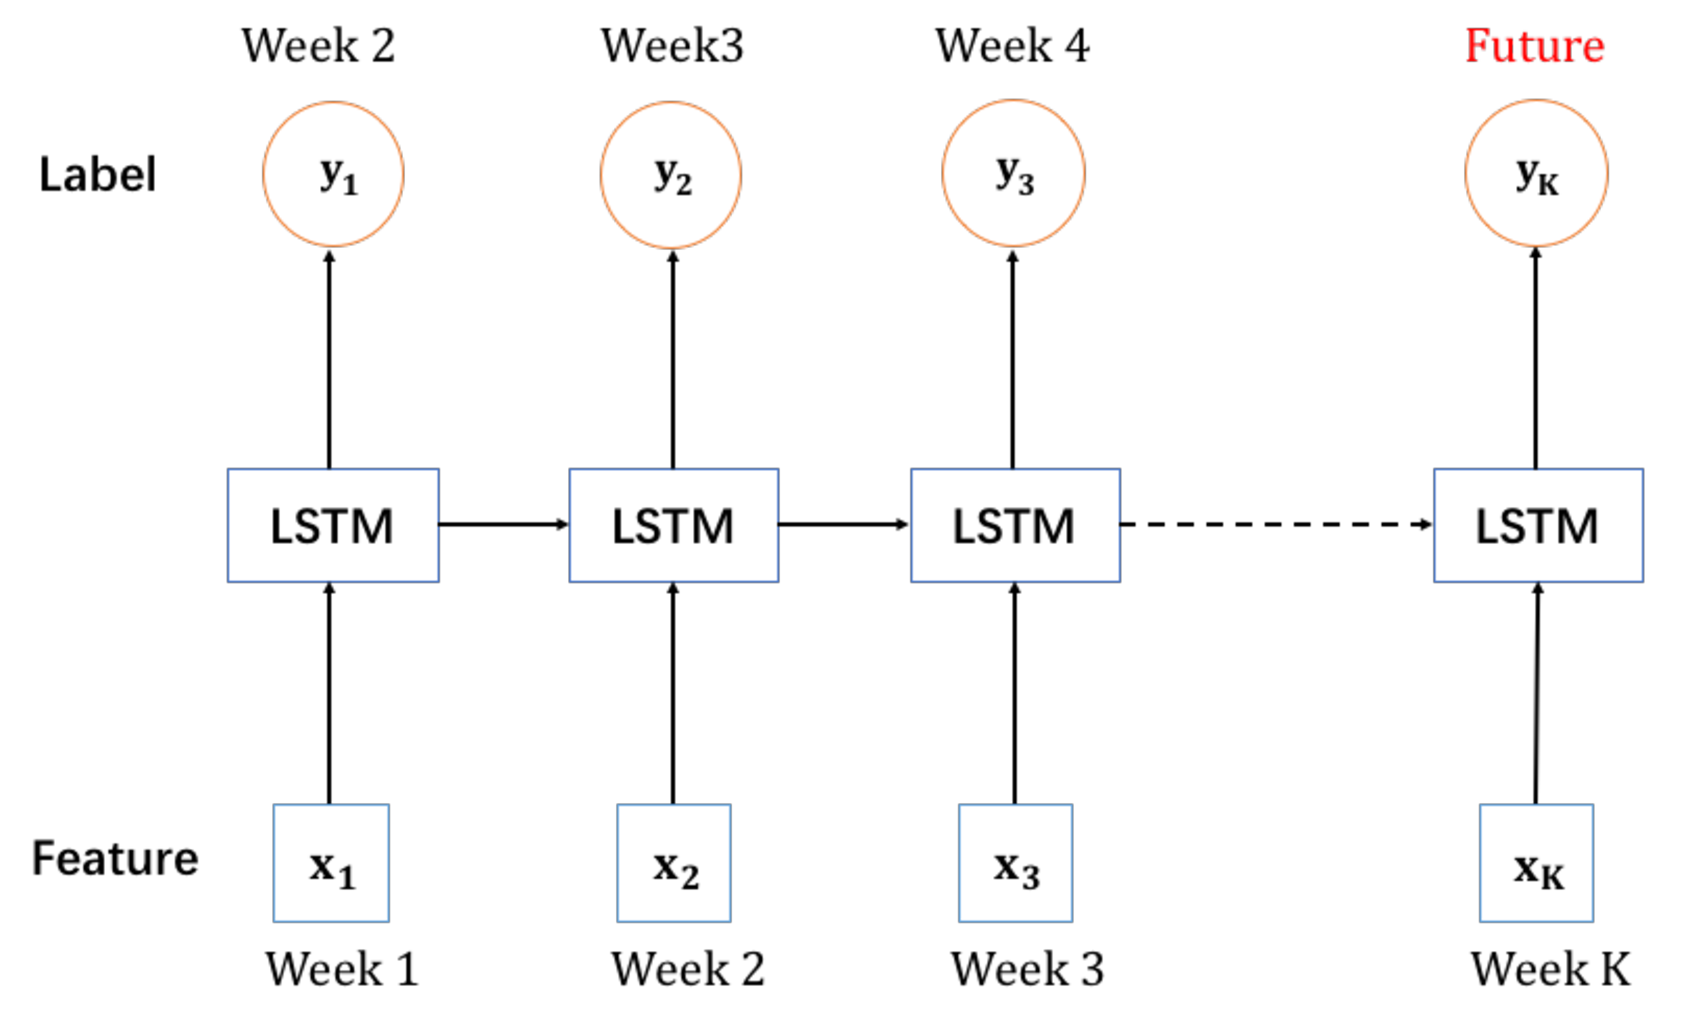
\includegraphics[width=6.4cm, height=3.5cm]{lstm.pdf}
	\caption{LSTM Model for Learning Temporal Patterns From Activity Sequence. We utilize user's Statistics Features in the former week to predict whether he would drop out in the latter week, while we use the features of the last week to predict her dropout in the \emph{future} period.}
	\label{fig:lstm}
\end{figure}
Besides simple statistics, we also adopt LSTM to learn the long-term behavior patterns from the historical activity sequence. LSTM  is an advanced type of recurrent neural network which leverages memory cells and gates to model long-term dependencies within a sequence \cite{Hochreiter1997Long}.  Specifically, Let $\mathbf{S}=(\mathbf{x}_1,\mathbf{x}_2,...,\mathbf{x}_K)$ denote the input sequence, where $\mathbf{x}_k$ is the input vector at position $k$. At each position $k$, there is a set of gate vectors, including input gate $\mathbf{i}_k$, forget gate $\mathbf{f}_k$ and output $\mathbf{o}_k$. It controls for which information should be forgotten, input and output, respectively. Moreover, LSTM adopts a memory cell state $\mathbf{C}_k$ to memorize the internal information at the current time and capture remote dependency. Based on gate vectors and memory cell, the output hidden state $\mathbf{h}_k$ at position $k$ is computed as follows. 
\begin{equation} \mathbf{f}_k = \sigma(\mathbf{W}_f\cdot [\mathbf{x}_k,\mathbf{h}_{k-1}]+\mathbf{b}_f) \end{equation}
\begin{equation} \mathbf{i}_k = \sigma(\mathbf{W}_i\cdot[\mathbf{x}_k,\mathbf{h}_{k-1}]+\mathbf{b}_i) \end{equation}
\begin{equation} \mathbf{C}_k = \mathbf{f}_k \odot \mathbf{C}_{k-1} + \mathbf{i}_t \odot \tanh(\mathbf{W}_c\cdot[\mathbf{x}_k,\mathbf{h}_{k-1}]+\mathbf{b}_c \end{equation}
\begin{equation} \mathbf{o}_k = \sigma(\mathbf{W}_o \cdot [\mathbf{x}_k,\mathbf{h}_{k-1}]+\mathbf{b}_o) \end{equation}
\begin{equation} \mathbf{h}_k = \mathbf{o}_k \odot \tanh(\mathbf{C}_k) \end{equation}
where $\sigma$ is the sigmoid function, $\odot$ is element-wise multiplication, and $\mathbf{W}, \mathbf{b}$ are weight matrices and weight vectors to be learned.\

LSTM is used to learn temporal patterns from user historical activity sequence. The basic idea is to regard this task as a sequential prediction problem and to employ LSTM to predict dropout by weeks.
Specifically, we first partition the \emph{history} period into $K$ weeks $(week_1,week_2,..., week_K)$. For each enrollment $(u,c)$, we utilize Statistics Features in $week_k(1 \le k \le K)$ to predict whether $u$ would drop out in the next week $week_{k+1}$. Whereas we use the features in the last week $week_K$ to predict the real dropout label, which indicates whether $u$ would drop out in the \emph{future} period. Here we use the Statistics Features of historical activity sequence in $k$-th week (described in the previous section), as the input vector $\mathbf{x}_k$ at position $k$. $y_k(1 \le k \le K)$ is defined below.\\
\begin{small}
$$y_k = 
	\begin{cases}
	\text{ 1 if user drops out in  } week_{k+1} \text{ else 0} & \makebox[45pt][r]{$1 \le k \le K-1$} \\
	\text{ 1 if user drops out in }  future \text{ period else 0} & \makebox[30pt][r]{$k=K$}
	\end{cases}
$$
\end{small}
\\
 %The first $K-1$ labels $(y_1, y_2,...,y_{K-1})$ indicate from week sequence $(W_2, W_3,...W_K)$  based on the dropout definition (in Section \ref{ProblemDef}) , whereas $y_{K}$ is the real label which indicates whether $u$ will dropout in $future$ periods. 
 For predicting $y_k(1 \le k \le K)$, the hidden state $\mathbf{h}_k$ at position $k$ is input into a logistics function:
 
\begin{equation}
\hat{y}_k=\frac{1}{1+e^{-\mathbf{w_y}^\mathsf{T} \mathbf{h}_k+b_y}}
 \end{equation}

\noindent where $\mathbf{w_y}$ is the weight vector and $b_y$ is the bias value.
The loss function is defined as:
\begin{equation}
\mathcal{L}(\Theta)= \sum_{k=1}^{K}[y_k\log(\hat{y}_k)+(1-y_k)\log(1-\hat{y}_k)]
\end{equation}
Figure \ref{fig:lstm} presents this model. We use the last prediction probability $\hat{y}_K$ and the last hidden state $\mathbf{h}_K$ as the LSTM Temporal Features.
\subsection{User-related Features}
	\label{sec:UFeat}
	This set of features is extracted from user-course enrollment graph and user profiles. We use these features to capture users' individual information. This type of features is denoted as  $\mathbf{Feat}_u$.\\
	
	\noindent \textbf{User Demographics}\\
    User Demographics (including \emph{gender, age, location, education level}) are extracted from user profiles, and we represent these attributes as a one-hot vector.\\
    
	\noindent \textbf{User Embedding}\\
	Though one-hot representation of a user's demographics can represent the user's necessary information, this method often suffers from sparsity problem in practice, and it could not capture sufficient information about users' preference. Thus we adopt network embedding algorithms to learn features from user-course enrollment graph $G_{uc}$. Similar to those in Section \ref{sec:influence}, we utilize DEEPWALK \cite{Perozzi:2014:DOL:2623330.2623732} to get distributed embedding for each node of $G_{uc}$, and user node embeddings are used as User Embedding features in our framework.\\

	\noindent \textbf{Influence features from friends}\\
	  As we analyzed in section \ref{sec:influence}, user $u$'s behavior in course $c$ is associated with her friends. Thus we design an algorithm to extract influence features from $u$'s friends who have enrolled the same course with her. Following the friends finding method in Section \ref{sec:influence}, for each $u\in \mathbb{U}_c$, we select top $10$ most similar users from her co-learning students set $\mathbb{U}_c-\{u\}$ as her friends. We denote $u$'s friends set as $\mathbb{S}_u=\{u_1, u_2...,u_{N_u}\}$, then the influence features $\mathbf{Feat}_{inf}$ can be calculated based on friends' activity features and similarity scores.
	\begin{equation}
		\mathbf{Feat}_{inf}(u) = \frac{\sum_{i=1}^{N_u} f_s(u, u_i)\mathbf{Feat}_{stat}(u_i)}{\sum_{i=1}^{N_u} f_s(u, u_i)}
	\end{equation}
	where $\mathbf{Feat}_{inf}(u)$ denotes the influence feature of $u$, $\mathbf{Feat}_{stat}(u_i)$ is the Statistics Features (Section \ref{sec:activityFeat}) of $u_i$, and $f_s$ is the similarity function, which is cosine function between the two node vectors.
	
\subsection{Course-related Features}
	\label{sec:CFeat}
	Similar to the User-related features, we also design a set of features to represent course specific information. This set of features is defined as $\mathbf{Feat}_c$.\\
	
	\noindent \textbf{Course Category}\\
	These features are acquired based on the courses categorization scheme provided by XuetangX, which categorizes the courses into twelve types (described in Section \ref{sec:XuetangX}). We also use a $12$-dim one-hot vector to represent each course's category in our framework.\\
	
	\noindent \textbf{Course Embedding}\\
	Similar to the User Embedding in Section \ref{sec:UFeat}, the embeddings of courses obtained from user-course enrollment graph are used as preference features from the perspective of course. \\
%from the dimension of course
